\documentclass[apectratio=43,unicode]{beamer}
\usetheme{Moscow}

\usepackage[utf8]{inputenc}
\usepackage[T2A]{fontenc}
\usepackage[main=russian,english]{babel}

\usepackage{amsmath,amssymb}

\renewcommand{\thefootnote}{\fnsymbol{footnote}}
\hypersetup{
	pdfauthor={Ivan Tsybulin}
}

\usepackage{euler}
\usepackage{mathtools}

\graphicspath{{images//}}

\title[Нелиненые уравнения]{Нелинейные алгебраические уравнения\\Системы алгебраических уравнений}
\author[Цыбулин И.В.]{Скалько Юрий Иванович\\
\textbf{Цыбулин Иван}
}
\date{}

\newcommand{\colorhref}[2]{\href{#1}{\textcolor{miptbase!30!black}{#2}}}

\begin{document}

\begin{frame}[plain]
\titlepage
\end{frame}

\section{ }

\def\A{{\bf A}}
\def\E{{\bf E}}
\def\F{{\bf F}}
\def\G{{\bf G}}
\def\H{{\bf H}}
\def\J{{\bf J}}
\def\x{{\bf x}}
\def\y{{\bf y}}
\def\b{{\bf b}}
\def\g{{\boldsymbol \varphi}}

\section{Нелинейные алгебраические уравнения}
\subsection{Скалярные уравнения}
\begin{frame}
\frametitle{Постановка задачи}
	Дана функция $f(x)$. Найти решение уравнения
	\[
	f(x) = 0
	\]

	В отличие от случая линейного уравнения, нелинейное уравнение может иметь сколько угодно корней,
	в том числе и не иметь их вовсе. Чтобы как-то конкретизировать корень, требуется дополнительно указать отрезок локализации.
	Задача формулируется в следующем виде: найти решение уравнения
	\[
	f(x) = 0, \quad x \in [a,b]
	\]
\end{frame}

\subsection{Уточнение локализации корня}
\begin{frame}
\frametitle{Метод дихотомии}
	Предположим, что непрерывная функция $f(x)$ принимает в концах отрезка $[a,b]$ разные по знаку значения.
	Пусть для определенности $f(a)<0,\, f(b)>0$. Иначе можно просто изменить знак у функции $f$
	Значит, на отрезке $[a,b]$ она принимает все значения от $f(a)$ до $f(b)$ включая и значение $0$.
	Таким образом, корень локализован на отрезке $[a,b]$. Разобьем его точкой $c = \frac{a+b}{2}$ на пару отрезков
	$[a,c]$ и $[c,b]$. Возможны варианты
	\begin{itemize}
		\item $f(c) = 0$. Корень найден - это точка $c$
		\item $f(c) < 0$. Поскольку $f(b) > 0$, то на отрезке $[c, b]$ должен быть корень $f(x) = 0$
		\item $f(c) > 0$. Поскольку $f(a) < 0$, то на отрезке $[a, c]$ должен быть корень $f(x) = 0$
	\end{itemize}
	Таким образом, задача свелась к такой же, но с меньшим отрезком.
\end{frame}

\begin{frame}
\frametitle{Скорость сходимости дихотомии}
	Сделав некоторое число делений отрезка пополам,
	можно получить хорошее приближение к решению уравнения. Поскольку длина отрезка на каждом шаге уменьшается в 2 раза
	$$b_n - a_n = \left(\frac{1}{2}\right)^n (b_0 - a_0)$$
	Корень уравнения расположен где-то на отрезке $[a_n, b_n]$, и можно написать
	$$
	\left|x^* - \frac{a_n+b_n}{2}\right| < \frac{|b_n - a_n|}{2} = |b_0 - a_0| \left(\frac{1}{2}\right)^{n+1}
	$$
	Метод сходится со скоростью геометрической прогрессии с показателем $q = \frac{1}{2}$
\end{frame}

\begin{frame}
\frametitle{Пример метода дихотомии}
	Рассмотрим в качестве примера функцию $f(x) = \tg \frac{x}{4} - 1$. Ее корни расположены в точках $x_k = (1 + 4k) \pi$
	Допустим, мы хотим найти численно корень $x_0 = \pi$. Необходимо найти отрезок локализации этого корня, на концах которого функция 
	принимает разные по знаку значения.

	Легко проверить, что $[3,4]$ удовлетворяет этому требованию.
	\begin{align*}
		[a_{0},b_{0}] &= [\underline{3.}0000000000, \underline{}4.0000000000]\\
		[a_{1},b_{1}] &= [\underline{3.}0000000000, \underline{3.}5000000000]\\
		[a_{2},b_{2}] &= [\underline{3.}0000000000, \underline{3.}2500000000]\\
		[a_{3},b_{3}] &= [\underline{3.1}250000000, \underline{3.}2500000000]\\
		&\vdots\\
		[a_{20},b_{20}] &= [\underline{3.141592}0258, \underline{3.141592}9794]\\
	\end{align*}
\end{frame}

\subsection{Простые итерации}
\begin{frame}
\frametitle{Метод простой итерации}
	Предположим, что уравнение $f(x) = 0$ удалось заменить эквивалентным ему уравнением $x = \varphi(x)$.
	Рассмотрим итерационный процесс
	\[
	x_{k+1} = \varphi(x_k)
	\]
	Рассмотрим, при каких условиях этот процесс сходится.
\end{frame}

\begin{frame}
\frametitle{Теорема Банаха о сжимающем отображении}
	На вопрос сходимости итерационного процесса $x_{k+1} = \varphi(x_k)$ отвечает следующая
	\begin{block}{Теорема(Банах,1922)}
		Если $\varphi(x): \mathbb{X} \mapsto \mathbb{X}$ задает сжимающее отображение, то есть существует $0 \leq q < 1$
		\[
		\rho(\varphi(x),\varphi(y)) \leq q \rho(x,y),
		\]
		то у отображения $\varphi(x)$ существует единственная неподвижная точка $x^* = \varphi(x^*)$ и
		\[
		x^* = \lim_{k \rightarrow \infty} x_k
		\]
	\end{block}
	То есть, если $\varphi(x)$ сжимающее отображение, то итерационный процесс сходится. Можно показать, что
	\[
	|x^* - x_k| < q^k |x^* - x_0|
	\]
\end{frame}

\begin{frame}
\frametitle{Сжимающие отображения}
	В качестве множества $\mathbb{X}$ может выступать, например, некоторый отрезок $[a,b]$.

	Заметим, что для метрики в $\mathbb{X}$ верно
	\[
	\rho(\varphi(x),\varphi(y)) = |\varphi(x)-\varphi(y)| \leq |\varphi'(\xi)| |x-y|  = |\varphi'(\xi)| \rho(x,y)
	\]

	При $|\varphi'(x)| \leq q < 1$ отображение сжимающее
	\[
	\rho(\varphi(x),\varphi(y)) \leq q \rho(x,y)
	\]
\end{frame}

\begin{frame}
\frametitle{Достаточное условие сжимаемости}
	Пусть $\varphi(x)$ отображает отрезок $[a,b]$ в себя и имеет на нем производную по модулю меньше $q < 1$.
	\begin{itemize}
		\item $\varphi([a,b]) \subset [a,b]$
		\item $\displaystyle \max_{x \in [a,b]}|\varphi'(x)| = q < 1$
	\end{itemize}
	Тогда $\varphi(x)$ задает на $[a,b]$ сжимающее отображение, а значит для нее итерационный процесс
	\[
	x_{k+1} = \varphi(x_k)
	\]
	сходится от любого начального приближения $x_0 \in [a,b]$ к неподвижной точке
	\[
	x^* = \varphi(x^*)
	\]
\end{frame}

\begin{frame}
\frametitle{Метод релаксации}
	Рассмотрим $f(x)$ такую, что $f(a) < 0, f(b) > 0$ и $f'(x) > 0$ на отрезке $[a,b]$.
	Построим $\varphi(x)$ следующим образом
	\[
	\varphi(x) = x - \tau f(x),\quad \tau > 0
	\]
	Тогда
	\[
	\varphi'(x) = 1 - \tau f'(x)
	\]
	Если взять $\tau < \frac{1}{\max f'(x)}$, то $0 \leq \varphi'(x) < 1$ и $\varphi(x)$ монотонно растет
	от $\varphi(a)$ до $\varphi(b)$. Поскольку $a < \varphi(a) \leq \varphi(b) < b$, такая функция $\varphi(x)$
	действительно отображает $[a,b]$ в себя и является сжимающей.

	Можно брать и другие значения $\tau$ вплоть до $\tau_{max} = \frac{2}{\max f'(x)}$, только сжимаемость требуется проверять
	непосредственно.
\end{frame}

\begin{frame}
\frametitle{Метод релаксации}
	Для примера возьмем то же уравнение $f(x) = \tg \frac{x}{4} - 1 = 0$. Возьмем следующую функцию
	\[
	\varphi(x) = x - \tau f(x) = x - \frac{3}{2}\left(\tg\frac{x}{4}-1\right)
	\]
	$\tau = \frac{3}{2} \approx \frac{2}{\max f'(x) + \min f'(x)}$ выбрано по аналогии с оптимальным
	значением $\tau$ для метода простой итерации для линейных систем $\tau_{opt} = \frac{2}{\lambda_1 + \lambda_n}$.
	При таком выборе $\tau$ максимум модуля производной $q = \max |\varphi'(x)|$ минимален, а значит процесс сходится быстрее всего.
	При данном $\tau$ $q \approx 0.30$, что меньше $0.5$ для метода дихотомии.

	Функция $\varphi(x)$ переводит отрезок $[3,4]$ в себя.

	Проделаем 20 итераций метода $x_{k+1} = \varphi(x_k)$
	\[x_{20} = \underline{3.141592653589}6458\]
\end{frame}

\begin{frame}
\frametitle{Метод простой итерации}
	Метод релаксации не всегда хорошо работает. Довольно часто можно
	подобрать другую функцию $\varphi(x)$, для которой процесс сходится быстрее.

	Рассмотрим уравнение $f(x) = \ln x + 2 - x = 0$.
	\begin{figure}%
	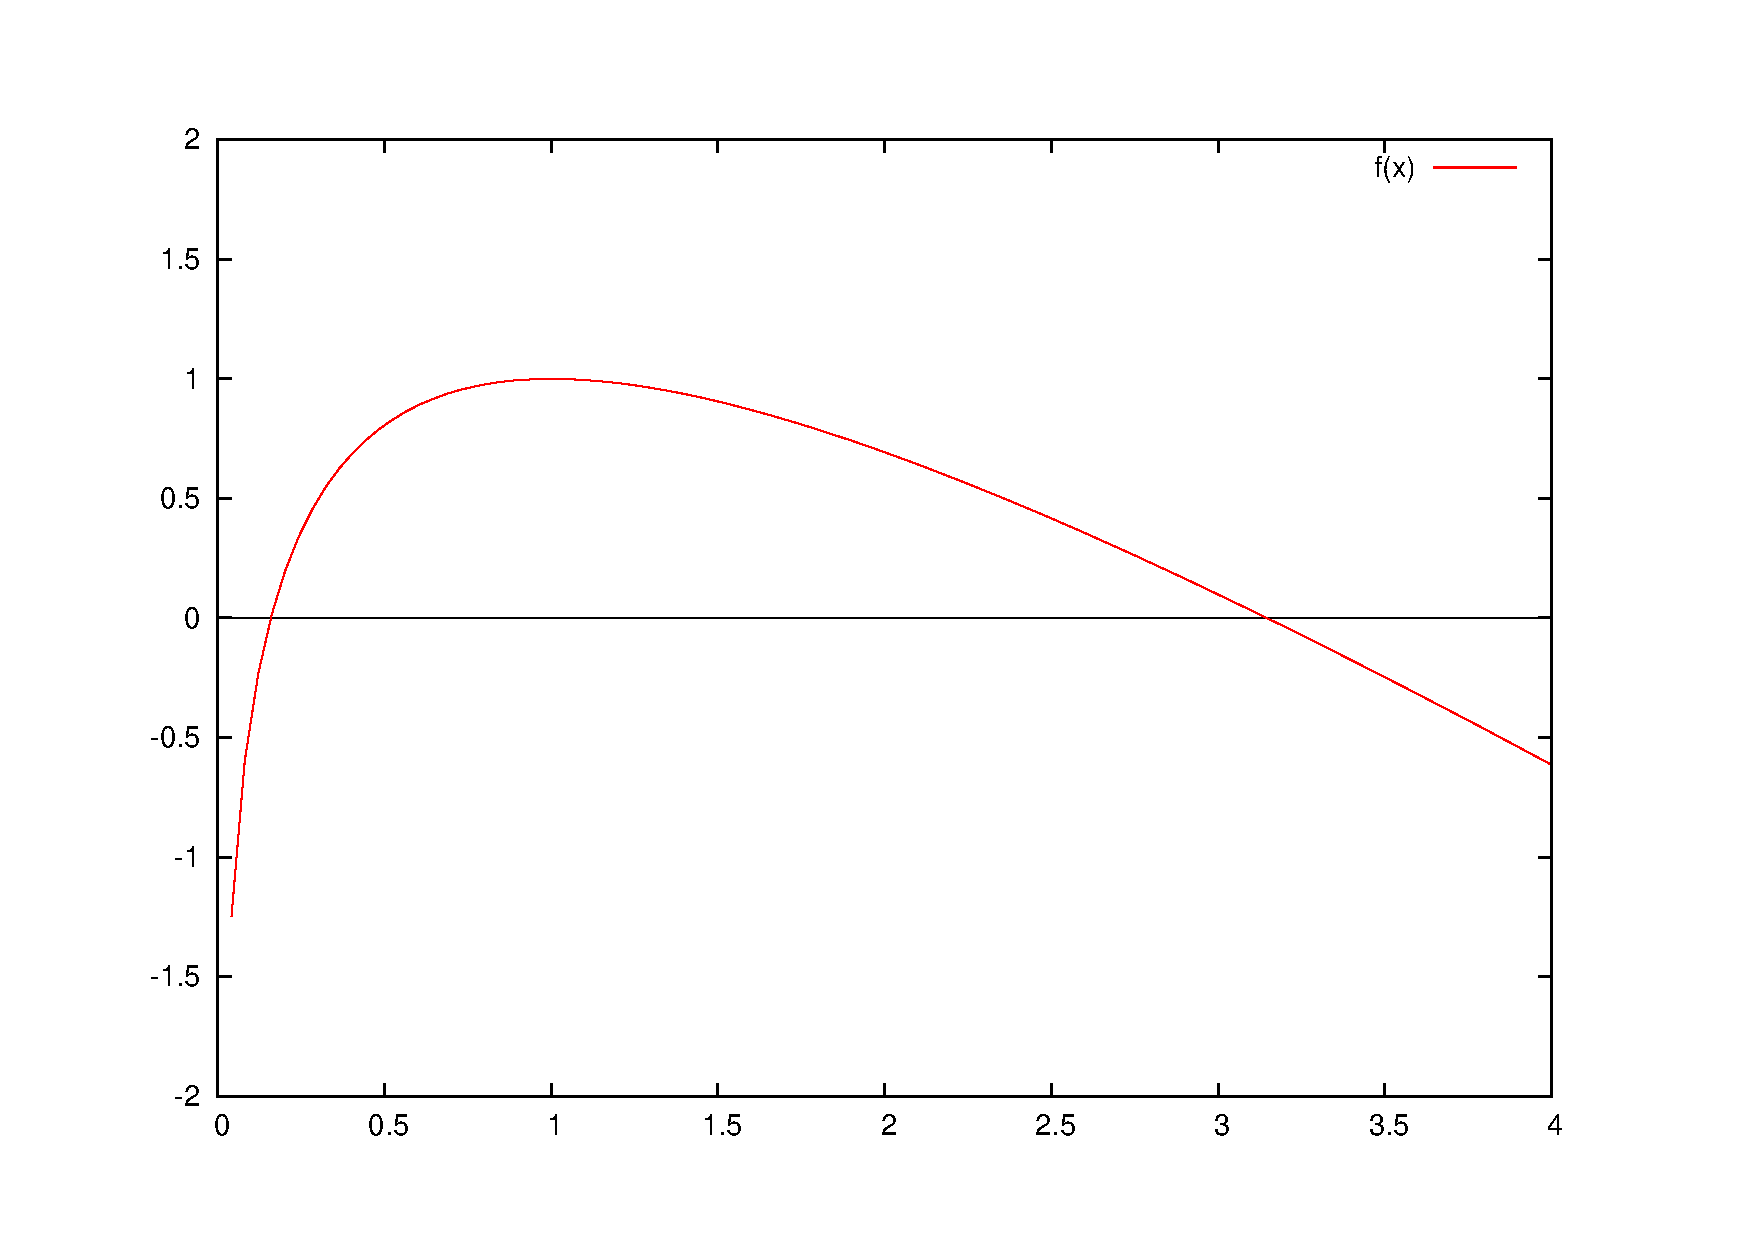
\includegraphics[height=0.6\textheight]{lnxmxp2.pdf}%
	\end{figure}
\end{frame}

\begin{frame}
\frametitle{Метод простой итерации}
	\[f(x) = \ln x + 2 - x = 0\]
	У данного уравнения два корня, первый лежит на отрезке $[e^{-2},e^{-1}]$, второй -- на $[3,e^2]$.
	\pause

	Возьмем $\varphi(x) = \ln x + 2$. Производная $\varphi'(x) = \frac{1}{x}$ по модулю меньше единицы при $x > 1$.

	Эта функция отображает отрезок $[3, e^2]$ в отрезок $[2 + \ln 3, 4] \subset [3,e^2]$, то есть задает на нем сжимающее отображение.
	\[
	q = \max_{x\in[3,e^2]} \left|\frac{1}{x}\right| = \frac{1}{3}
	\]

	Метод $x_{k+1} = \varphi(x_k)$ будет сходиться к корню из отрезка $[3,e^2]$.
\end{frame}

\begin{frame}
\frametitle{Метод простой итерации}
	\begin{figure}%
	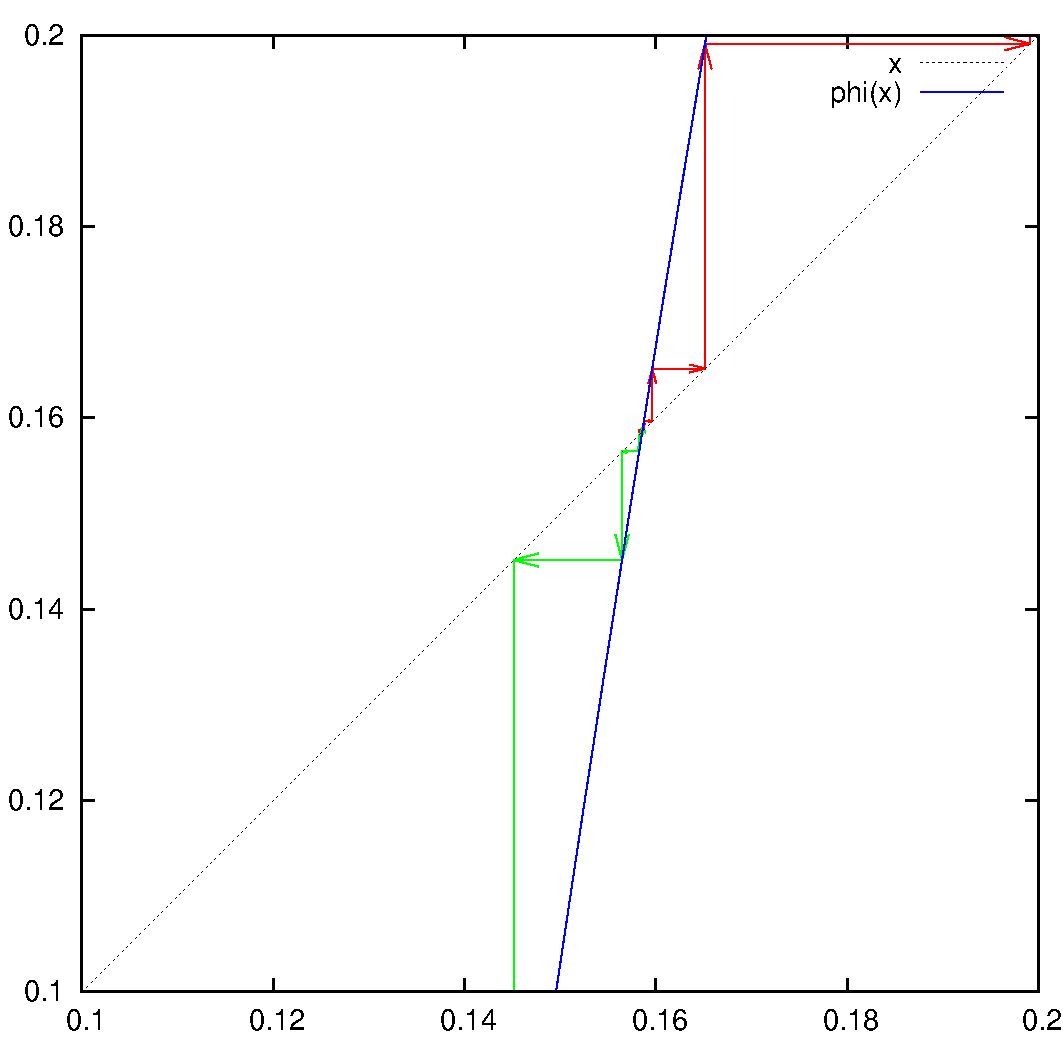
\includegraphics[width=0.5\columnwidth]{si2.pdf}%
	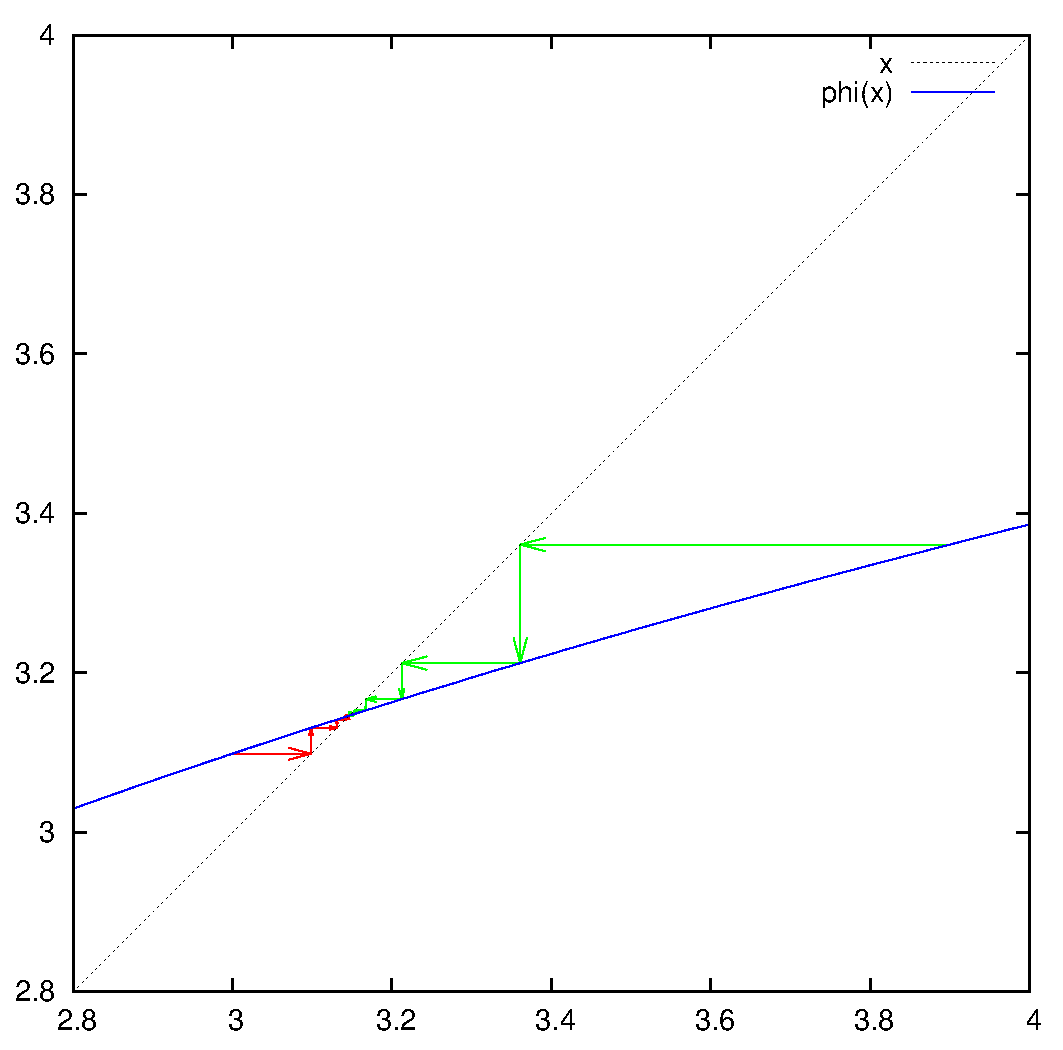
\includegraphics[width=0.5\columnwidth]{si.pdf}%
	\caption[]{Поведение метода в окрестности первого и второго корня}
	\end{figure}
\end{frame}

\begin{frame}
\frametitle{Метод простой итерации}
	\[f(x) = \ln x + 2 - x = 0\]

	Построим для первого корня метод простой итерации на отрезке $[e^{-2}, e^{-1}]$.
	\[
	\varphi(x) = x - \tau f(x)
	\]
	При оптимальном по скорости сходимости
	$\tau = \frac{2}{e^2-1 + e-1} \approx 0.25$
	функция $\varphi(x)$ осуществляет сжимающее отображение отрезка $[e^{-2},e^{-1}]$ в себя, причем коэффициент сжмания $q \approx 0.58$.
	Видно, что метод сходится довольно медленно, в данном случае метод дихотомии оказался бы быстрее.
\end{frame}

\begin{frame}
\frametitle{Метод простой итерации}
	Вспомним случай $\varphi(x) = \ln x + 2$. Метод расходился, убегая от корня, даже при очень близких начальных значениях.
	\pause

	<<Развернем>> направление итераций. Рассмотрим вместо
	\[
	x_{k+1} = \varphi(x_k)
	\]
	процесс
	\[
	x_{k} = \varphi(x_{k+1}), \quad x_{k+1} = \varphi^{-1}(x_k)
	\]
	Обратная функция $\varphi^{-1}(x) = e^{x-2}$.
	Она отображает внутрь себя отрезок $[e^{-2}, e^{-1}]$ и ее производная $\varphi'(x) = e^{x-2}$ на этом отрезке ограничена по модулю $q = 0.20$.

	Этот метод сходится в три раза быстрее метода простой итерации с оптимальным параметром и $q = 0.58$!
\end{frame}

\subsection{Метод Ньютона}
\begin{frame}
\frametitle{Метод Ньютона}
	В основе метода Ньютона лежит замена нелинейного уравнения $f(x) = 0$ приближенным линейным уравнением.
	Разложим $f(x)$ в окресности точки $x_k$ в ряд Тейлора, отбросив все члены кроме первых двух.
	\[
	0 = f(x) \approx f(x_k) + f'(x_k)(x - x_k)
	\]
	Линейное уравнение легко решается $x = x_k - \frac{f(x_k)}{f'(x_k)}$. Возьмем это решение в качестве нового приближения к решению $f(x) = 0$
	\[
	x_{k+1} = \varphi(x_k) = x_k - \frac{f(x_k)}{f'(x_k)}
	\]
\end{frame}

\begin{frame}
\frametitle{Сходимость метода Ньютона}
	Существует окрестность точки $x^*$, в которой $|\varphi'(x)| < 1$.
	\begin{block}{Теорема(Канторович)}
		Если существуют константы $A,B,C$ такие, что на отрезке $[a,b]$
		\begin{itemize}
			\item $\frac{1}{|f'(x)|} < A$, то есть $f'(x)$ ограничена и не равна $0$
			\item $|\frac{f(x)}{f'(x)}| < B$, то есть $f(x)$ ограничена
			\item $|f''(x)| \leq C \leq \frac{1}{2AB}$
			\item $|a-b| < \frac{1}{AB}\left(1-\sqrt{1-2ABC}\right)$
		\end{itemize}
		Тогда на отрезке $[a,b]$ есть корень уравнения $f(x) = 0$, и метод Ньютона с $x_0 = \frac{a+b}{2}$ сходится к нему с квадратичной скоростью
		\[
		|x_n - x^*| \leq \frac{B}{2^{n-1}} (2ABC)^{2^{n-1}} \leq D q^{2^n}
		\]
	\end{block}
\end{frame}

\begin{frame}
\frametitle{Квадратичная сходимость}
	В отличие от ранее рассмотренных методов, метод Ньютона сходится квадратично. Это значит что на каждой итерации точность не просто увеличивается, умножаясь на константу,
	а возводится в квадрат.
	Сравните линейную сходимость
	\[
	|x^* - x_k| \leq q |x^* - x_{k-1}|
	\]
	и квадратичную
	\[
	|x^* - x_k| \leq q |x^* - x_{k-1}|^2
	\]

	На практике квадратичная сходимость выражается в \emph{удвоении} на каждом шаге количества правильных знаков.
	В случае линейной сходимости каждая итерация \emph{добавляла} несколько правильных знаков.
\end{frame}

\begin{frame}
\frametitle{Сходимость метода Ньютона}
	Чтобы получить на практике квадратичную сходимость необходимо удовлетворить нескольким условиям из теоремы.
	Но, как правило, условиям теоремы удовлетворяет довольно малый отрезок $[a,b]$, и чтобы реально получить быструю сходимость
	требуется выбрать очень хорошее начальное приближение.

	Если нарушать условия теоремы, и выбрать плохое начальное приближение, возможна расходимость или не сходимость метода Ньютона
\end{frame}

\begin{frame}
\frametitle{Сходимость метода Ньютона}
	\begin{figure}%
	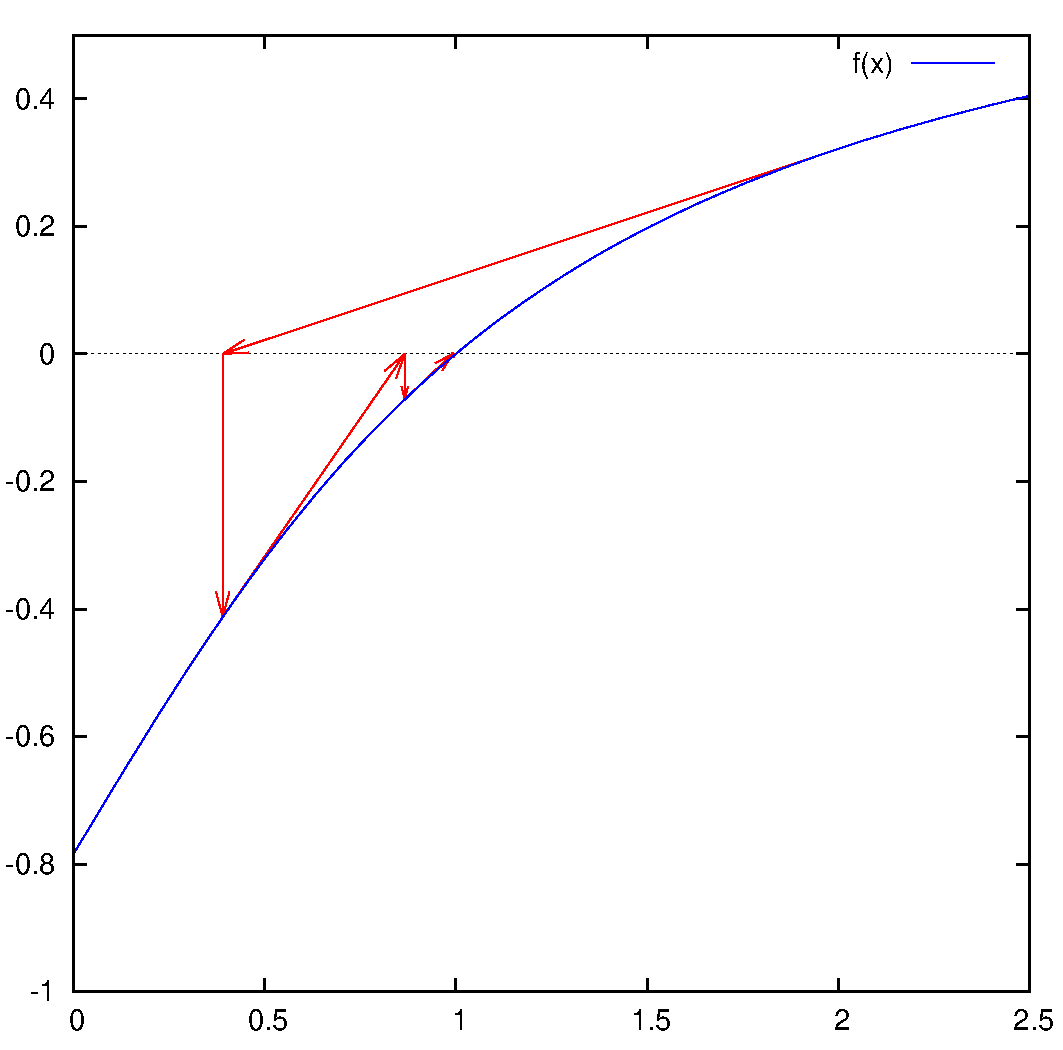
\includegraphics[width=0.5\columnwidth]{nw.pdf}%
	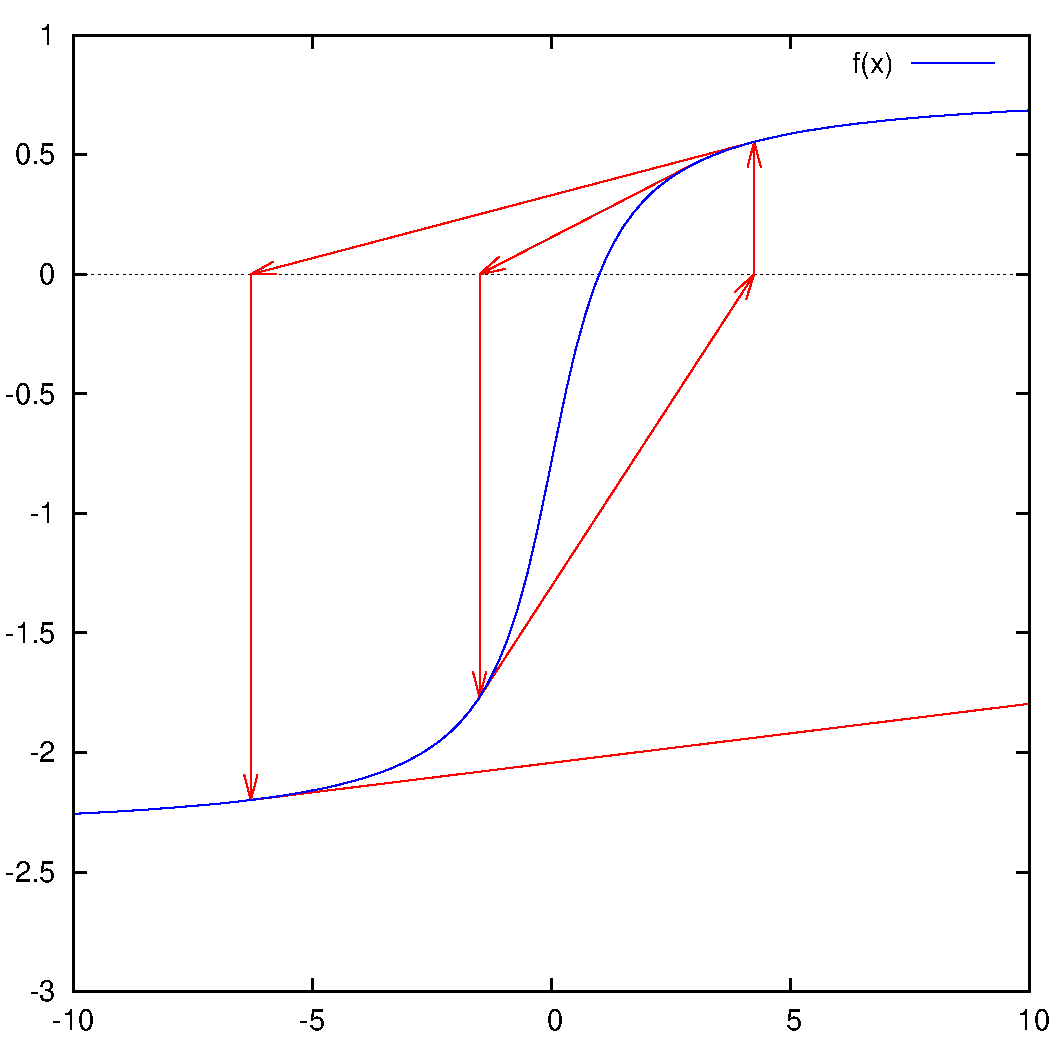
\includegraphics[width=0.5\columnwidth]{nw2.pdf}%
	\caption{Поведение метода Ньютона при различных начальных приближениях}%
	\end{figure}
\end{frame}

\subsection{Метод секущих}
\begin{frame}
\frametitle{Метод секущих}
	В случаях, когда непосредственно нахождение производной функции $f(x)$ затруднительно, прибегают к методу секущих.
	В нем вместо точного значения производной используется разностное отношение
	\[
	x_{k+1} = x_k - \frac{x_k - x_{k-1}}{f(x_k) - f(x_{k-1})} f(x_k)
	\]

	Метод позволяет сохранить квадратичную сходимость метода Ньютона, но может испытывать численные неустойчивости в окрестности корня.
	К тому же метод стал трехшаговым, то есть $x_{k+1}$ вычисляется через пару $x_k$ и $x_{k-1}$, и методу необходимо два начальных приближения $x_0$ и $x_1 \neq x_0$.
\end{frame}

\subsection{Системы нелинейных уравнений}
\begin{frame}
\frametitle{Постановка задачи}
	Дана система алгебраических уравнений
	\begin{align*}
	f_1(x_1,x_2,\dots,x_n) &= 0\\
	f_2(x_1,x_2,\dots,x_n) &= 0\\
	&\vdots\\
	f_m(x_1,x_2,\dots,x_n) &= 0\\
	\end{align*}
	или в векторной форме
	\[
	\F(\x) = 0, \qquad \F: \mathbb{R}^n \mapsto \mathbb{R}^m
	\]
	Требуется найти решение, локализованное в области $G \subset \mathbb{R}^n$.

	Система алгебраических уравнений может как иметь так и не иметь решений вне зависимости от 
	соотношения между числом неизвестных $n$ и уравнений $m$.
\end{frame}

\begin{frame}
\frametitle{Сжимающие отображения}
	Теорема Банаха может применяться и в этом случае. Если $\g(\x)$ задает сжимающее отображение 
	замкнутой области $G$ в себя ($\g(G) \subset G$) и
	\[
	\|\g(\x) - \g(\y)\| \leq q \|\x - \y\|
	\]
	то последовательность $\x_{k+1} = \g(\x_k)$ будет сходится к неподвижной точке $\x^* = \g(\x^*)$.
\end{frame}

\begin{frame}
\frametitle{Сжимающее отображение}
	В многомерном случае есть теорема, дающая достаточное условие сжимаемости отображения $\g$
	\begin{block}{Теорема}
		Если $G$ - выпуклая область, все производные $\frac{\partial \varphi_i}{\partial x_j}$
		равномерно непрерывны на $G$ и норма матрицы Якоби
		$$
		\J = \left[\frac{\partial \varphi_i}{\partial x_j} \right]
		$$
		не превосходит $q < 1$, то отображение является сжимающим в $G$
	\end{block}
	В случае, когда $G$ - компакт, равномерная непрерывность производных следует из непрерывности.

	Отличие от одномерного случая в том, что вместо условия $|\varphi'(x)| \leq q < 1$ теперь используется $\|\J\| \leq q < 1$
\end{frame}

%\begin{frame}
%\frametitle{Оптимизационные методы}
%	Для любой системы $\F(\x) = 0$ можно построить функцию $\Phi(\x) = \left(\F(\x), \F(\x)\right)$.
%	Эта функция неотрицательна $\Phi(\x) \geq 0$, а ее минимум $\Phi(\x) = 0$ достигается как раз в точке $\x^*$ где $\F(\x^*) = 0$.
%
%	\[
%	\nabla \Phi(\x) = 2\left(\frac{\partial \F(\x)}{\partial \x}\right)^T \F(\x)
%	\]
%
%	Для поиска минимума функции $\Phi(\x)$ можно применять различные методы оптимизации, например,
%	метод градиентного спуска или метод сопряженных градиентов.
%\end{frame}

\begin{frame}
\frametitle{Метод Ньютона}
	Метод Ньютона можно применять и в многомерном случае при выполнении условия $n = m$.

	\[
	\x_{k+1} = \x_k - \left[\frac{\partial \F(\x_k)}{\partial \x}\right]^{-1} \F(\x_k)
	\]

	Практически все свойства одномерного метода Ньютона без изменений переносятся на многомерный случай. Заметим, что в данном случае приходится
	на каждом шаге решать систему линейных уравнений с матрицей $\frac{\partial \F(\x_k)}{\partial \x}$.
\end{frame}

%\begin{frame}
%\frametitle{Метод продолжения по параметру}
%	Иногда бывает легко найти решение системы $\G(\x) = 0$ ``похожей'' на систему $\F(\x) = 0$, но решение $\G(\x)$ не является достаточно
%	хорошим приближением, чтобы метод Ньютона для системы $\F$ сошелся.
%
%	Рассмотрим систему $\H(\x, \lambda)$ с параметром $\lambda \in [0,1]$.
%	\[
%	\H(\x, \lambda) = \lambda \F(\x) + (1-\lambda) \G(\x)
%	\]
%
%	При $\lambda = 0$ система $\H$ совпадает с $\G$, а при $\lambda = 1$ --- с $\F$. Решение системы $\H(\x, 0) = \G(\x)$ известно. Можно
%	рассмотреть функцию $\x(\lambda)$ --- решение системы $\H$ при заданном $\lambda$. $\x(0)$ известно --- это решение $\G(\x)$. Обозначим его $\x_0$
%\end{frame}
%
%\frametitle{Метод продолжения по параметру}
%\begin{frame}
%	\[
%	\H(\x, \lambda) = \lambda \F(\x) + (1-\lambda) \G(\x)
%	\]
%
%	Поскольку $\x(\lambda)$ --- решение $\H$, то
%	\[
%	0 = \H(\x(\lambda), \lambda)
%	\]
%	Продифференцируем это выражение по $\lambda$
%	\[
%	0 = \frac{\partial \H}{\partial \x} \frac{d \x(\lambda)}{d \lambda} + \frac{\partial \H}{\partial \lambda}
%	\]
%	Отсюда
%	\[
%	\frac{d \x(\lambda)}{d \lambda} = \left(\lambda \F_\x(\x) + (1-\lambda) \G_\x(\x)\right)^{-1} (\G(\x) - \F(\x))
%	\]
%	Дополнив это уравнение условием $\x(0) = \x_0$, получаем задачу Коши для функции $\x(\lambda)$.
%\end{frame}

\begin{frame}
\frametitle{Метод Зейделя}
	Примечательно, но идея, которая использовалась для решения СЛАУ методом Зейделя переносится и на СНАУ
	\begin{align*}
	f_1(\fbox{$x_{k+1,1}$}; x_{k,\phantom{+1}2};\dots;x_{k,\phantom{+1}n}) &=0\\
	f_2(x_{k+1,1};\fbox{$x_{k+1,2}$}; \dots; x_{k,\phantom{+1}n}) &=0\\
	f_3(x_{k+1,1};x_{k+1,2};\dots; x_{k,\phantom{+1}n}) &=0\\
	&\vdots\\
	f_n(x_{k+1,1};x_{k+1,2};\dots;\fbox{$x_{k+1,n}$}) &= 0
	\end{align*}
	Если решать уравнения сверху вниз, то каждое уравнение является уравнением с одной неизвестной.
\end{frame}

\begin{frame}[plain]
  \begin{center}
  {\Huge Спасибо за внимание!}
  \vspace{8ex}

  Цыбулин Иван

  e-mail: \colorhref{mailto:tsybulin@crec.mipt.ru}{tsybulin@crec.mipt.ru}
  \end{center}
\end{frame}

\end{document}
